\chapter{Requirements Specification}
In this chapter we shall outline the system requirements. The first section shows a \gls{uml} use case diagram, used to explore and convey uses of the system in order to help derive requirements. The second section defines the requirements outright.

\section{Use Case}

\subsection{Use Case Diagram}

\begin{figure}[H]
    \centering
    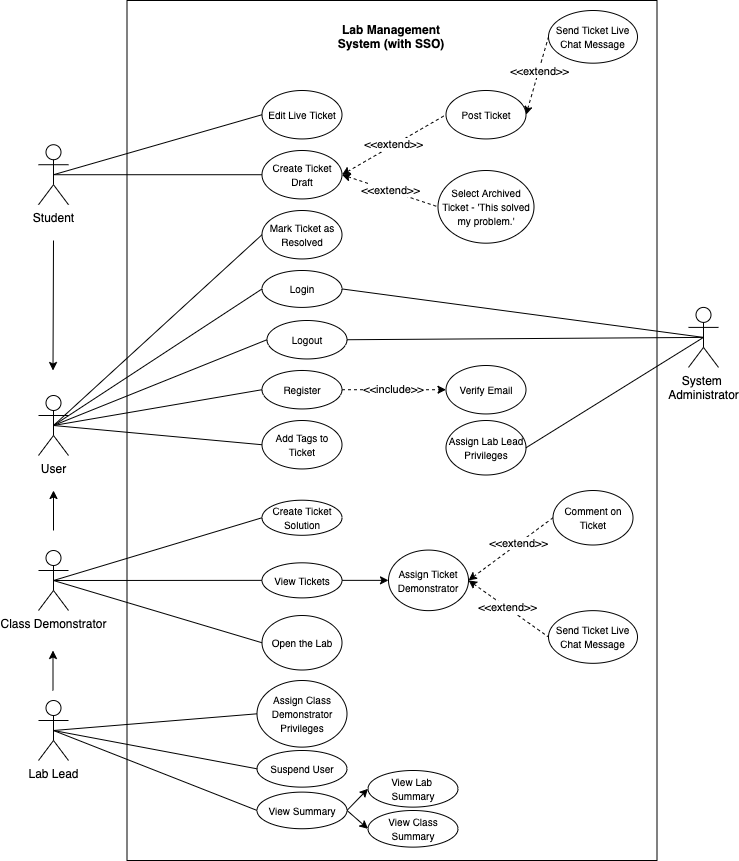
\includegraphics[width=\textwidth]{5requirements/images/useCase.png}
    \caption{Use case diagram for lab management system.}
    \label{fig:useCase}
\end{figure}

\subsection{Use Case Specifications}

\subsection*{`Create Ticket Draft' Use Case Specification}
\begin{table}[H]
\centering
 \begin{tabular}{p{0.27\linewidth}  p{0.67\linewidth}}
 \textbf{Use case name} & \textbf{Post Ticket}  \\
 Use case ID & 1\\
 Brief Description & A student creates a ticket draft on the system.\\
 Preconditions & The student is a registered and verified, the lab is open.\\
 Primary actors & Student. \\
 Secondary actors & \textbf{None.} \\
 Successful end condition & A new live ticket is posted onto the system for class demonstrators to view. \\
 Failed end condition & The ticket listing is rejected. \\
 Main flow & Steps:\\
 & 1. The use case starts when a student tries to visit the `post a ticket' page.\\
 & 2. The system checks that the user is logged in as a registered, verified account with student role privileges. \\
 & 3. The `post a ticket' page is opened. \\
 & 4. The student inputs the details of the issue - associated module, relevant practical or worksheet, the issue category and a description issue.\\
 & 5. The student submits the information. \\
 & 6. The system checks that the student has not posted a ticket in the last 3 minutes. \\
 & 7. The system checks that the ticket does not contain offensive or abusive language. \\
 & 8. The system checks that no archived, resolved tickets are highly similar to the draft ticket.\\
 & 9. The new ticket is posted on the application.\\

 Extension & Step\hspace{0.3cm} Branching Action \\
 & 2.1 \hspace{0.5cm}The user is not logged in as a registered, verified student. \\
 & 2.2 \hspace{0.5cm}Access to the `post a ticket' page is denied. \\
 & 6.1 \hspace{0.5cm}The student has posted a ticket in the last 3 minutes. \\
 & 6.2 \hspace{0.5cm}The system does not post the ticket, shows an error message modal. \\
 & 7.1 \hspace{0.5cm} The ticket contains offensive or abusive language.\\
 & 7.2 \hspace{0.5cm} The system does not post the ticket, shows an error message modal and logs the ticket for review by a lab lead.\\
 & 8.1 \hspace{0.5cm} The draft ticket is highly similar to one or more archived, resolved tickets.\\
 & 8.2 \hspace{0.5cm} The system allows the student to view the similar ticket(s).\\
 & 8.3 \hspace{0.5cm} The student selects `this solved my problem' on a ticket.\\
 & 8.4 \hspace{0.5cm} The system records the selection of the archived ticket and discards the student's draft ticket.\\
 & 8.3.1 \hspace{0.5cm} The student selects `this does not help'.\\
 & 8.3.2 \hspace{0.5cm} The new ticket is posted on the application.\\
 
\end{tabular}
\end{table}

\newpage
\subsection*{`Resolve Ticket' Use Case Specification}
\begin{table}[H]
\centering
 \begin{tabular}{p{0.27\linewidth}  p{0.67\linewidth}}
 \textbf{Use case name} & \textbf{Resolve Ticket}  \\
 Use case ID & 2\\
 Brief Description & A class demonstrator resolves a student's issue ticket.\\
 Preconditions & The ticket is live and not assigned to any class demonstrators.\\
 Primary actors & Class Demonstrator. \\
 Secondary actors & Student. \\
 Successful end condition & The ticket is marked as resolved. \\
 Failed end condition & The ticket is mark as closed but unresolved. \\
 Main flow & Steps:\\
 & 1. The use case starts when a class demonstrator attempts to visit the live tickets page.\\
 & 2. The system checks that the user is logged in as a registered, verified account with class demonstrator role privileges. \\
 & 3. The live ticket page is opened and shows a queue of all unresolved, not closed tickets that were posted in the current lab. \\
 & 4. The class demonstrator selects a ticket in the queue.\\
 & 5. The class demonstrator assigns themselves to the ticket. \\
 & 6. The class demonstrator sends the student a live chat, either explaining the solution, asking for more information or requesting a video chat. \\
 & 7. The class demonstrator solves the student's problem and marks the issue ticket as resolved. \\
 & 8. The class demonstrator is given the option to store a solution to the problem on the system.\\
 & 9. The ticket is archived on the system.\\

 Extension & Step\hspace{0.3cm} Branching Action \\
 & 2.1 \hspace{0.5cm}The user is not logged in as a registered, verified class demonstrator. \\
 & 2.2 \hspace{0.5cm}Access to the live ticket page is denied. \\
 & 7.1 \hspace{0.5cm} The class demonstrator cannot solve the problem.\\
 & 7.2 \hspace{0.5cm} The ticket is closed, marked unresolved, and the system logs the ticket for review by a lab lead.\\
  
\end{tabular}
\end{table}

\section{System Requirements}

\paragraph{Stakeholders} The system has four different types of stakeholder - the students, the class demonstrator, the lab lead and the system administrator. The system administrator role was designed with the intention of being managed by course organisers.

\subsection{TODO? User Stories}

\newpage
\subsection{Functional Requirements}

The following requirements list is prioritised using the \gls{moscow} technique, reducing the indecision associated with simpler prioritisation. They are split with the view that no more than 60\% of effort should be spent on `Must Have' requirements of the project, along with a sensible pool of `Could Haves' of around 20\% effort \cite{dsdm}.

TODO: sort table by priority?
TODO: later in project, make sure table fits properly

\begin{table}[H]
\small
\begin{tabular}{|p{0.05\linewidth} | p{0.78\linewidth} |p{0.09\linewidth}|}
 \hline
 \textbf{ID} & \textbf{Details} & \textbf{Priority} \\
 \hline
 
 \multicolumn{3}{c}{\textit{\textbf{Account Requirements}}}\\
 
 \hline
 F-01 & \textit{Description:} The system shall allow students to register on the system by providing a verified student email address and a password. & M\\
  \cline{2-2}
  & \textit{Rationale:} Students must be able to sign up using only a school email address, which they can verify access to, to register on the system. & \\

  
   \hline\hline
 F-02 & \textit{Description:} The system should allow students to sign in using the Shibboleth \gls{sso} system used by the school. & W\\
  \cline{2-2}
  & \textit{Rationale:} Students can only log in if Shibboleth authenticates them, making the system more secure, reliable and meaning authentication is centralised to align with other school systems. & \\

  
     \hline\hline
 F-03 & \textit{Description:} Lab leads shall be able to assign class demonstrator role to users. & M\\
  \cline{2-2}
  & \textit{Rationale:} This allows class demonstrator accounts to be created without allowing regular students to attempt to class create demonstrator accounts. & \\

  
       \hline\hline
 F-04 & \textit{Description:} System administrators shall be able to assign lab lead role to users. & M\\
  \cline{2-2}
  & \textit{Rationale:} This allows lab lead accounts to be created. & \\
  \hline
  
   \multicolumn{3}{c}{\textit{\textbf{Ticket Requirements}}}\\
  
 \hline
 F-05 & \textit{Description:} Whilst the lab is open, students shall be able to create `tickets' by providing information on the module code, practical or workshop number, issue category and issue description. & M\\
  \cline{2-2}
  & \textit{Rationale:} This creates a record of the issue that the student is having for the class demonstrators to interact with. & \\

  
 \hline\hline
 F-06 & \textit{Description:} Students should be able to add tags to their own tickets which associate them with related tickets. & S\\
  \cline{2-2}
  & \textit{Rationale:} This allows students to give more clarification about the nature of the problem, create links with similar tickets (which they can view) and also help the system recommendation algorithm recommend similar past tickets. & \\

  
    \hline\hline
 F-07 & \textit{Description:} The system should recommend similar archived tickets before students post their tickets. & C\\
  \cline{2-2}
  & \textit{Rationale:} This allows students to scan archived tickets, checking if any will help resolve their issue, before they post a live ticket that demonstrators need to deal with. & \\
  
      \hline\hline
 F-08 & \textit{Description:} The system should keep a record of which archived tickets students have selected (`this solved my problem') before deleting the original ticket draft. & C\\
  \cline{2-2}
  & \textit{Rationale:} This allows lad leads and demonstrators to get information on issues which multiple students have had. & \\
  
   \hline\hline
 F-09 & \textit{Description:} Class demonstrators shall be able to assign themselves to tickets. & M\\
  \cline{2-2}
  & \textit{Rationale:} This allows demonstrators to keep track of, and indicate to other demonstrators, which issues they are working on or have completed. & \\

  
  \hline\hline
 F-10 & \textit{Description:} Class demonstrators shall be able to comment on tickets. & S\\
  \cline{2-2}
  & \textit{Rationale:} This allows demonstrators to make notes on the issues and initiate contact with the students, although actual communication would primarily be done outside the system. & \\

    \hline\hline
 F-11 & \textit{Description:} Class demonstrators shall be able to close tickets. & S\\
  \cline{2-2}
  & \textit{Rationale:} This allows demonstrators to mark tickets as no longer being `live' - either marking them as resolved or closed. & \\

  
      \hline\hline
 F-12 & \textit{Description:} Students should be able to close tickets. & S\\
  \cline{2-2}
  & \textit{Rationale:} This allows students to remove their issues from the queue if they have solved the problem themselves. & \\
\hline



  \end{tabular}
\end{table}

\begin{table}[H]
\small
\begin{tabular}{|p{0.05\linewidth} | p{0.78\linewidth} |p{0.09\linewidth}|}
  
          \hline
 F-13 & \textit{Description:} Class demonstrators should be able to `open' the lab, allowing tickets to be created by students. & S\\
  \cline{2-2}
  & \textit{Rationale:} This allows demonstrators to prevent help requests outwith lab hours. & \\

  
\hline\hline
 F-14 & \textit{Description:} Lab leads should be able to disable user accounts from the system. & C\\
  \cline{2-2}
  & \textit{Rationale:} This allows lab leads to remove users who are no longer students, demonstrators or alternatively for inappropriate behaviour or posting excessively. & \\
 
 \hline\hline
 F-15 & \textit{Description:} The system should not allow offensive or abusive content to be posted. & C\\
  \cline{2-2}
  & \textit{Rationale:} Prevents offensive behaviour. & \\
 
 \hline\hline
 F-16 & \textit{Description:} The system should not allow students to have more than one live ticket. & C\\
  \cline{2-2}
  & \textit{Rationale:} This prevents individual students from posting an excessive number of tickets on the system. TODO: should this be 3 minutes? limit to number of req per lab instead??? & \\
 
  \hline\hline
 F-17 & \textit{Description:} The system should allow students to edit and update their live tickets. & C\\
  \cline{2-2}
  & \textit{Rationale:}  This allows users to provide more information on a ticket to improve demonstrators ability to help them. & \\
 
   \hline\hline
 F-18 & \textit{Description:} The system shall have an integrated live chat feature on each ticket that has a demonstrator assigned. & S\\
  \cline{2-2}
  & \textit{Rationale:} This allows students and demonstrators to briefly discuss minor issues or to arrange communication outside the system. & \\

   \hline\hline
 F-19 & \textit{Description:} The system should have some form of video chat option on each ticket that has a demonstrator assigned. & C\\
  \cline{2-2}
  & \textit{Rationale:} This allows students and demonstrators to resolve the problem raised by the ticket, removing any human error associated with looking the student up on another system - as well as reducing time spent doing so. & \\

   \hline\hline
 F-20 & \textit{Description:} The system should allow class demonstrators to post a `solution' for ticket. & C\\
  \cline{2-2}
  & \textit{Rationale:} This allows demonstrators to store solutions with archived tickets, useful for future reference when archived tickets are recommended as similar to future students' tickets. & \\

   \hline\hline
 F-21 & \textit{Description:} The system should prompt class demonstrators to provide solutions for archived tickets which have repeatedly been marked by students as similar to their own tickets. & C\\
  \cline{2-2}
  & \textit{Rationale:} This encourages demonstrators to provide solutions for more common problems, ensuring the recommendation system will be useful and therefore reduce the number of new tickets being created. It is also useful for reference by other class demonstrators. & \\

  
     \hline\hline
 F-22 & \textit{Description:} The system should give some indication to students of how busy the current lab session is or how many tickets are ahead of them in the queue. & S\\
  \cline{2-2}
  & \textit{Rationale:} This allows students to appreciate the amount of wait time that a response may require. & \\

     \hline\hline
 F-23 & \textit{Description:} The system shall allow students to specify their location for in-person labs. & S\\
  \cline{2-2}
  & \textit{Rationale:} This allows the tool to be used for management of in-person labs, as well as labs which are both in-person and have virtual participants. & \\
 
      \hline\hline
 F-24 & \textit{Description:} The system should allow students to attach files to their tickets. & S\\
  \cline{2-2}
  & \textit{Rationale:} This allows demonstrators to study, understand and potentially solve issues quickly before they need to contact the student. & \\
  \hline
 
 \end{tabular}
\end{table}
 
 \begin{table}[H]
\small
\begin{tabular}{|p{0.05\linewidth} | p{0.78\linewidth} |p{0.09\linewidth}|}
 
  \multicolumn{3}{c}{\textit{\textbf{Summary Requirements}}}\\
  
          \hline
 F-25 & \textit{Description:} The system should show class demonstrators and lab leads a `timeline' of all actions on the system - such as lab opening, ticket posting, ticket commenting, ticket resolution and lab closing. & C\\
  \cline{2-2}
  & \textit{Rationale:} This allows demonstrators and lab leads to quickly scan recent activity, as well as helping demonstrators to quickly find recent tickets or comments. & \\
  
\hline\hline
 F-26 & \textit{Description:} Lab leads shall be able to view lab summaries which provide statistics about the amount of tickets resolved, who resolved tickets and how long tickets remained unresolved in each individual lab. & M\\
  \cline{2-2}
  & \textit{Rationale:} This allows lab leads to review the efficiency of the ticketing system in the lab. & \\

 \hline\hline
 F-27 & \textit{Description:} Lab leads shall be able to view class summaries which provide statistics about the amount of tickets resolved, who resolved tickets and how long tickets remained unresolved for all labs in a given class. & M\\
  \cline{2-2}
  & \textit{Rationale:} This allows lab leads to review the efficiency of the ticketing system in the class. & \\
  \hline
  
\end{tabular}
\end{table}

\subsection{Non-Functional Requirements}

\begin{table}[H]
\small
\begin{tabular}{|p{0.07\linewidth} | p{0.78\linewidth} |p{0.09\linewidth}|}
 \hline
 \textbf{ID} & \textbf{Details} & \textbf{Priority} \\
 
 \hline
   \multicolumn{3}{c}{\textit{\textbf{Usability Requirements}}}\\
 \hline
 
   NF-01 & \textit{Description:} 95\% of students should be able to create a ticket in less than 5 minutes on the first attempt. & M \\
  \cline{2-2}
  & \textit{Rationale:} The system should be intuitive, quick and easy to use. & \\

   \hline\hline
      NF-02 & \textit{Description:} 95\% of class demonstrators should be able to resolve a ticket, in the correct way (for example, marking the problem as resolved), in less than 1 minute on the first attempt. & M \\
  \cline{2-2}
  & \textit{Rationale:} The system should be intuitive, quick and easy to use. & \\
   \hline
     
     \multicolumn{3}{c}{\textit{\textbf{Security Requirements}}}\\
     
     \hline
 NF-03 & \textit{Description:} Data shall be encrypted. & M\\
  \cline{2-2}
  & \textit{Rationale:} Data needs to be protected from hostile users. & \\
  
    \hline\hline
 NF-04 & \textit{Description:} Data shall be stored securely. & M\\
  \cline{2-2}
  & \textit{Rationale:} Data needs to be protected from hostile users. & \\
  
      \hline\hline
 NF-05 & \textit{Description:} The system shall anonymise (and archive for future reference) all resolved tickets. & M\\
  \cline{2-2}
  & \textit{Rationale:} This allows the system to show users the archived tickets without processing or storing any personal data. & \\
  
      \hline\hline
 NF-06 & \textit{Description:} The system shall only alloq class demonstrators (and lab leads) to view live tickets and names of students. & M\\
  \cline{2-2}
  & \textit{Rationale:} This addresses privacy concerns arising from students being able to view other students' names and tickets. & \\
\hline
  
    \multicolumn{3}{c}{\textit{\textbf{Performance Requirements}}}\\
    
  \hline
   NF-07 & \textit{Description:} Class demonstrator ticket assignment shall be processed and updated for other users within 0.1s. & S \\
  \cline{2-2}
  & \textit{Rationale:} Slow assignment processing and updating could result in issues with conflicting assignment and demonstrators working on the same ticket. & \\
 
   \hline\hline
   NF-08 & \textit{Description:} Resolution of tickets shall be processed and updated for other users within 1s. & S \\
  \cline{2-2}
  & \textit{Rationale:} Ticket resolution should be processed reasonably quickly to prevent lab leads following up tickets resolved by demonstrators or demonstrators following up tickets resolved by students. & \\
  \hline
  
      \multicolumn{3}{c}{\textit{\textbf{Dependability Requirements}}}\\
  
   \hline
   NF-09 & \textit{Description:} The System shall achieve 99\% up time. & S \\
  \cline{2-2}
  & \textit{Rationale:} Since students rely on the labs for help and they are only open for a small amount of time, it is critical that down time during the lab window is reduced. & \\
\hline
   
\multicolumn{3}{c}{\textit{\textbf{Space Requirements}}}\\
   
   \hline
   NF-10 & \textit{Description:} The system should be able to store at least 100,000 tickets. & S \\
    \cline{2-2}
  & \textit{Rationale:} Since there are many labs for each module, which involves multiple practicals, it is important that the archive is capable of storing tickets for future reference. & \\
 \hline

\end{tabular}
\end{table}


